\chapter{Results}
\label{cha:Results}

This chapter presents the results of the experiments conducted in this project. The first three experiments were designed to answer the research questions posed in chapter \ref{cha:ResearchGoals} specifically. 

The experiments were conducted using the policy that was developed as a result of the parameter experimentation \ref{sec:most_successful_policy}. This policy was trained exclusively on hard tracks with all light settings. The histogram equalization preprocessing step was used during training.


\section{Eval for question 1}

The trained policy was evaluated on tracks of all difficulty settings with the standard light setting using the Basic Evaluation algorithm \ref{sec:basic_evaluation_algorithm} with 100 episodes per setting. The success rates for the different difficulty settings are shown in figure \ref{fig:result_success_rates_standard}. Example videos of the agent's behaviour during evaluation can be found in the appendix \ref{cha:example_videos}.

\subsection{Experiment Results}

\begin{figure}
    \centering
    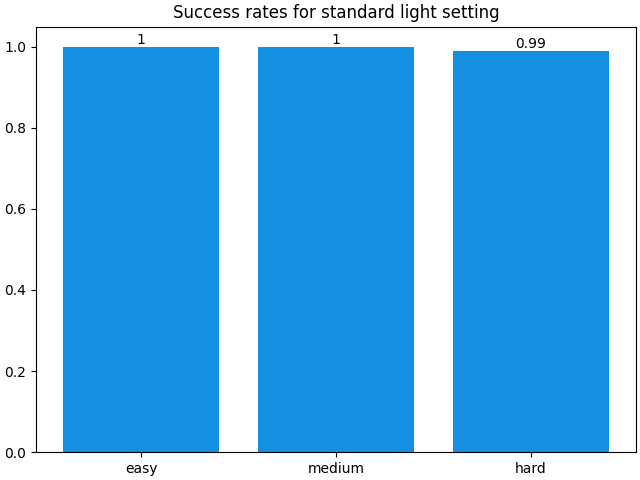
\includegraphics[width=0.45\textwidth]{Bilder/notebook_images/hardDistanceMixedLight_eval_standard_success_rates_barplot.png}
    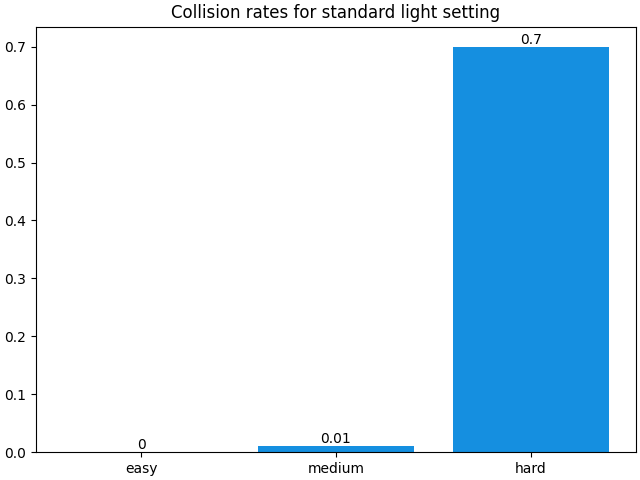
\includegraphics[width=0.45\textwidth]{Bilder/notebook_images/hardDistanceMixedLight_eval_standard_collision_rates_barplot.png}
    \caption{Success and collision rates for standard light setting.}
    \label{fig:result_success_rates_standard}
\end{figure}


The policy completed the easy, medium and hard tracks with a succes\_rate of 100\%, 100\% and 99\%. 
The collision\_rates were 0\%, 1\% and  70\%. Especially for the hard difficulty setting, the agent does not avoid collisions completely. 

The analysis of successful episodes with collisions shows that these collisions are only minor collisions. The agent passes the goals very close to the goal post that is closer to the arena middle \ref{fig:agent_behaviour}. This often results in collisions with the goal obstacles at its side.

\begin{figure}
    \centering
    \subfigure[Agent passes the goal close to the arena middle]{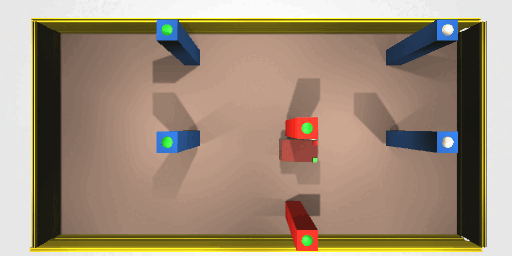
\includegraphics[width=0.45\textwidth]{Bilder/example_goal_passing_close_to_middle.png}}
    \subfigure[Agent may collide with goal post at the side]{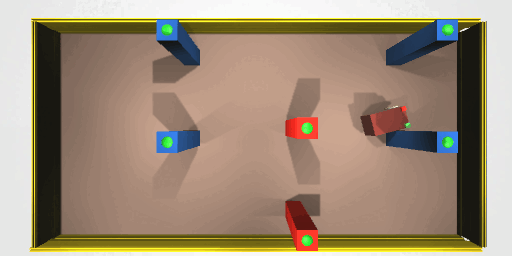
\includegraphics[width=0.45\textwidth]{Bilder/example_minor_collision_topview_frame_1295.png}}
    \caption{Goal passing behaviour of the trained agent}
    \label{fig:agent_behaviour}
\end{figure}

The unsuccessful episodes of hard tracks were analyzed to determine why the agent does not reach 100\% success rates. The analysis showed that the agent has frontal collisions with the first goal post at the agents side \ref{fig:unsuccessful_episodes}. This occurs only when the agent is spawned with an extreme rotation. The agent cannot complete the tracks in about 40\% of episodes with the maximum rotation of $15^{\circ}$.

\begin{figure}
    \centering
    \subfigure[Agent is spawned with extreme rotation]{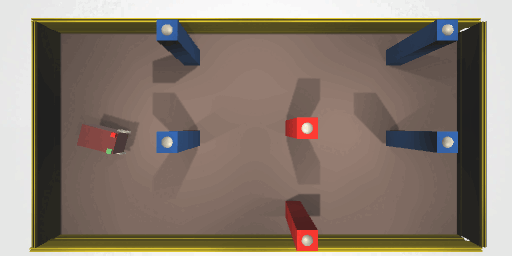
\includegraphics[width=0.3\textwidth]{Bilder/extremeSpawnRot_agent_initial.png}}
    \subfigure[Agent approaches first goal post]{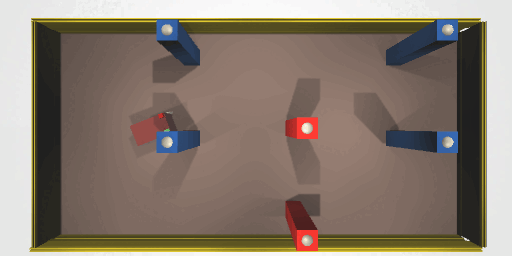
\includegraphics[width=0.3\textwidth]{Bilder/extremeSpawnRot_agent_turns.png}}
    \subfigure[Agent collides with first goal post and remains stuck]{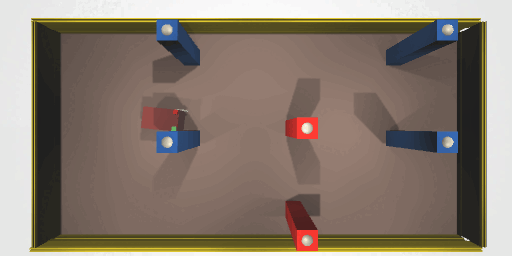
\includegraphics[width=0.3\textwidth]{Bilder/extremeSpawnRot_agent_collides.png}}
    \caption{Analysis of unsuccessful episodes}
    \label{fig:unsuccessful_episodes}
\end{figure}



\subsection{Conclusion}

The trained policy is able to complete all difficulty levels very reliably.

The policy was trained on the difficult setting only. The policy did not see easy and medium difficulty parcours before the evaluation. The policy is able to generalize to tracks of lower difficulty.

\section{Eval for question 2}

The most succesfull model was used to evaluate the agent's performance under different light settings. The agent was evaluated on the standard, dark and bright light settings. Each combination of difficulty and light setting was evaluated with the Basic Evaluation Algorithm for 100 episodes. The success rates for the different light settings are shown in figure \ref{fig:result_success_rates_lightSettings}.


\subsection{Experiment Results}

\begin{figure}
    \centering
    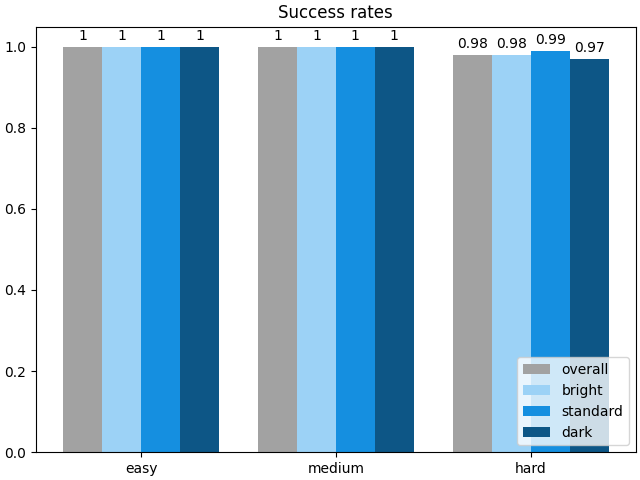
\includegraphics[width=0.45\textwidth]{Bilder/notebook_images/hardDistanceMixedLight_eval_all_success_rates_barplot.png}
    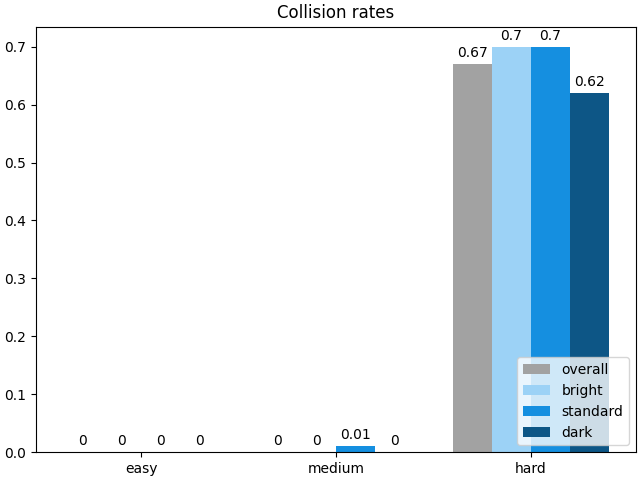
\includegraphics[width=0.45\textwidth]{Bilder/notebook_images/hardDistanceMixedLight_eval_all_collision_rates_barplot.png}
    \caption{Success and collision rate comparisons for light settings.}
    \label{fig:result_success_rates_lightSettings}
\end{figure}

The success rates for all light and difficulty settings are very high at above 95\%. The agent completed the easy and medium tracks with a success rate of 100\%. The light setting had no influence on the success\_rate for the easy and medium tracks.
The evaluations for the bright and dark light settings show slight decreases in performance compared to the standard light setting for hard tracks. The success\_rate of hard tracks in the bright and dark light setting was 98\% and 97\%.

The collision rates are very low for the easy and medium tracks. All tracks in these settings were solved without collisions except for the medium tracks with the standard light setting. This medium standard evaluation had a collision rate of 1\%.
The collision rates for the hard tracks are quite high at 70\% for the standard light setting. The bright and dark light settings are very high as well with 70\% and 62\%.

Across all light and difficulty settings the overall success rate is almost 100\% and the overall collision rate is 22\%.

\subsection{Conclusion}

The policy was able to complete the parcours very reliably under the different light settings. The light setting only had a minor impact on the success rate.
Furthermore the different light settings did not lead to an overall increase in collisions.

The developed policy was trained following the experiments in the previous chapter. The policy used the histogram equalization preprocessing step and mixed light settings during training. Using these settings the policy was able to learn to navigate the tracks with all light conditions.


\section{Eval for Question 3 - Replays}

The most successful model was used to record replays of the agent's behaviour. This most successful model used a $fixedTimestepLength$ of $0.3$ seconds. This means the hardware has to able to make a decision every $0.3$ seconds to be considered fast enough.

Five episodes were recorded for each difficulty and light setting combination. As expected from the previous evaluations of the policy, the replay episodes had a very high success\_rate of 100\%. The recorded episodes were then replayed on the Nvidia Jetbot. The time it took to replay the episodes was measured \ref{fig:result_replay_times}. The policy outputs from the replay were compared to the policy outputs from the recordings \ref{fig:result_replay_outputs}. The differences are caused by the hardware and software differences between the training and the replay environment.


\begin{figure}
    \centering
    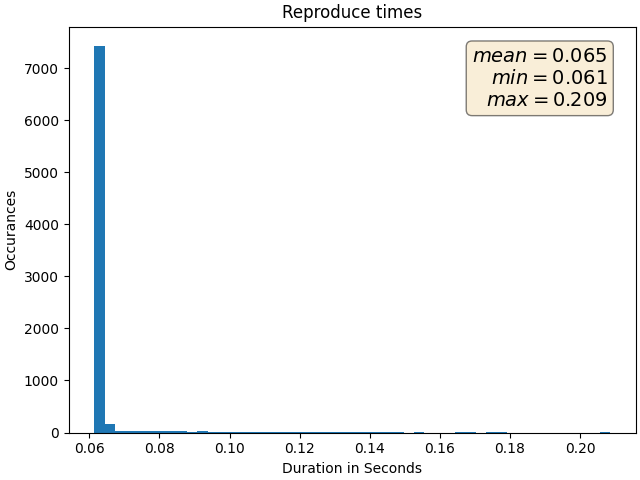
\includegraphics[width=0.5\textwidth]{Bilder/notebook_images/replay_times.png}
    \caption{Replay times on jetbot hardware}
    \label{fig:result_replay_times}
\end{figure} % a chart showing the replay times (max, min, mean)


\begin{figure}
    \centering
    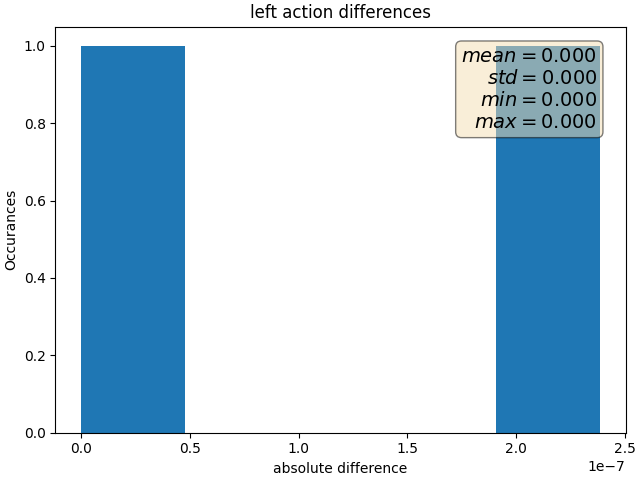
\includegraphics[width=0.45\textwidth]{Bilder/notebook_images/replay_outputs_action_left.png}
    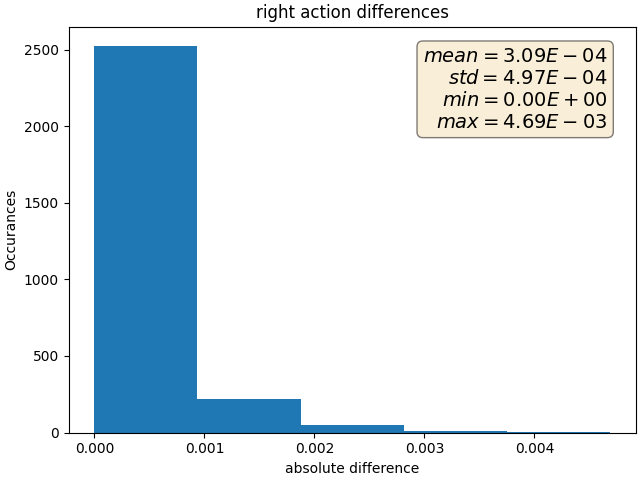
\includegraphics[width=0.45\textwidth]{Bilder/notebook_images/replay_outputs_action_right.png}
    \caption{Differences in policy outputs between recordings and replays on jetbot hardware}
    \label{fig:result_replay_outputs}
\end{figure} % a chart showing the replay outputs


\subsection{Experiment Results}

\paragraph{Replay times}

The replay times for the recordings on jetbot hardware are shown in figure \ref{fig:result_replay_times}. The maximum duration was $0.216$ seconds. The mean is much lower at $0.067$ seconds. The plot shows that the maximum duration was an extreme outlier.
Given the $fixedTimestepLength$ of $0.3$ seconds and the maximum duration of $0.216$ seconds, the hardware is fast enough to replay the episodes. This leaves at least $0.084$ seconds for the agent to recieve an image from the camera and send the new instruction to the motors.

The cameras used in the nvida jetbot are capable of capturing images with a resolution of $1280x720$ pixels at $60$ frames per second. This means the camera can capture an image every $0.0166$ seconds. The hardware is quick enough to compute actions in real time.

% times replay hardDistanceMixedLight: min 0.06319522857666016, mean 0.06662133265668013, max 0.21592259407043457

\paragraph{Policy Outputs}

The policy outputs from the recordings and the replays on jetbot hardware are nearly identical. The differences are shown in figure \ref{fig:result_replay_outputs}. The outputs were reproduced very closely. The maximum difference was $4.69e-03$.  This is difference is negligeable compared to the range of policy outputs $[-1,1]$.

% left action differences min [0.], max [0.00433731], mean 0.00030147546203806996, std 0.0004885991802439094
% right action differences min [0.], max [0.00468674], mean 0.00030857478850521147, std 0.000496754830237478

\subsection{Discussion}

The jetbot hardware is capable enough to compute the policy in real time. The differences of the policy outputs between the recordings and the replays are very small, the policy outputs were reproduced very closely. This suggests the differences in hardware and software do not impact the policy significantly.

\section{Other experiments}

\subsection{Sampling mode performance test}
\label{ref:sampling_mode_test_results}

The sampling mode performance test uses the Basic evaluation algorithm to evaluate an agent with derministic and non-deterministic sampling for each difficulty level. The success rates for the two sampling modes are compared to determine if the agent's performance is influenced by the sampling method. The sampling mode test was executed for all agents during the experimentation phase of this project using standard light.

\paragraph{Results}
The tests showed that the difference in performance for the sampling modes was very small for the trained policies. The results showed empirically that non-deterministic sampling leads to better success rates. Nevertheless some policies performed slightly worse using the non-deterministic sampling mode. The success rate was on average 1.7\% higher when using non-deterministic sampling. The biggest difference was 2.6\% for the medium difficulty setting \ref{fig:deterministic_check_result}.

\begin{figure}
    \centering
    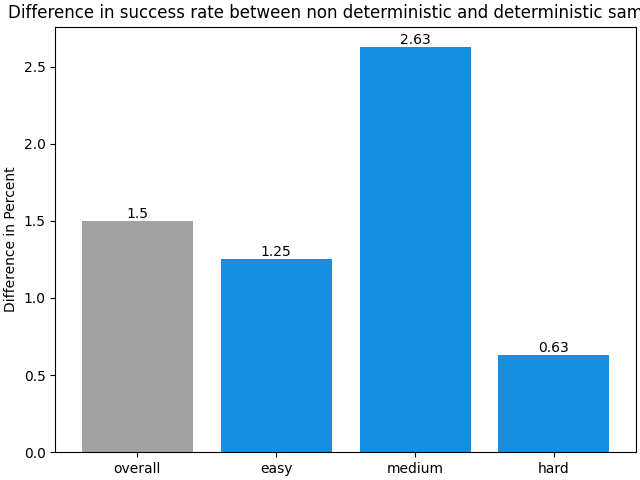
\includegraphics[width=0.8\textwidth]{Bilder/notebook_images/deterministic_check_results.png}
    \caption{Results of the deterministic check across all evaluations during the experimentation phase}
    \label{fig:deterministic_check_result}
\end{figure}

\paragraph{Discussion}
The test indicates that the non-deterministic sampling mode performes better, although the differences in performance are quite small. Given these results, the main evaluations for question 1 and 2 were conducted with non-deterministic sampling.

\subsection{Test identical start conditions}

The environment is not 100\% deterministic. This is due to the environment implementation in Unity. The environment uses physics simulations which are not deterministic. In addition the agent's actions are sampled non-deterministically during the evaluation.
This means that the same start conditions of an episode may result in different trajectories and results. This test evaluates the impact of the non-deterministic environment and sampling on the agent's behaviour. 
The trained agent is placed in the same start conditions for 100 episodes and the trajectories are compared. The starting conditions entail the selected track, light condition and the agent's starting rotation.

\paragraph{Results}

identical start conditions result in over 90\% identical trajectories for hard tracks

\paragraph{Discussion}

--> nice


\subsection{Fresh Observations Test}

The policy was trained to not use fresh observations \ref{sec:non_blocking_step_calls} with a fixed step duration of 0.3 seconds. The policy input recieves the observation from the start of the previous step as input. The policy input essentially lags 0.3 seconds behind the environment state. This saves processing time during training and evaluation. Alternatively a policy can be run with the $use\_fresh\_obs$ parameter. This makes the policy request a fresh observation from the Unity simulation.

The Fresh Observations Test analyses whether switching the trained policy to use fresh observations improves the performance. The policy is evaluated with fresh observations and without fresh observations for each difficulty level using the Basic Evaluation Algorithm \ref{sec:basic_evaluation_algorithm}. The success rates are compared to determine if fresh observations improve the agent's performance.

\paragraph{Results}

\begin{figure}
    \centering
    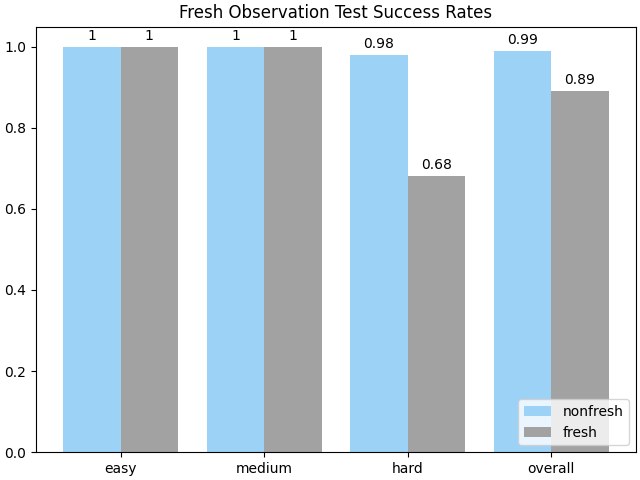
\includegraphics[width=0.8\textwidth]{Bilder/notebook_images/hardDistanceMixedLight_eval_freshNonFresh_success_rates_barplot.png}
    \caption{Success rates for policy evaluation using fresh and non-fresh observations}
    \label{fig:fresh_observations_test_result}
\end{figure}

The results show that the policy performs similar for the easy and medium settings. The success rates are 100\% for both fresh and non-fresh observations. The hard setting shows a strong decrease in performance when using fresh observations. The success rate drops from 98\% to 68\% \ref{fig:fresh_observations_test_result}.

The evaluations using fresh observations also take longer. The Basic Evaluation Algorithm's per call time for the fresh observations is about 20 minutes compared to 17 minutes for the non-fresh observations. The evaluation using fresh observations is slower because the policy has to request a fresh observation from the Unity simulation. This takes additional time.


\paragraph{Discussion}

The policy was trained using non-fresh observations. The policy's performance decreases for hard tracks when it is evaluated using fresh observations.
This suggests that the policy has learned to work with the lag of 0.3 seconds between the environment state and input to the policy. The policy's performance decreases when the lag is removed.

The test confirms that the $use\_fresh\_obs$ parameter should not be changed after the training has been completed.


\subsection{Jetbot generalization}

The policy was trained using the DifferentialJetBot shown in figure \ref{fig:jetbots}. The Jetbot Generalization test evaluates the same policy using the FourWheelJetBot. The policy is only evaluated on the standard light setting to save time.

\paragraph{Results}

\begin{figure}
    \centering
    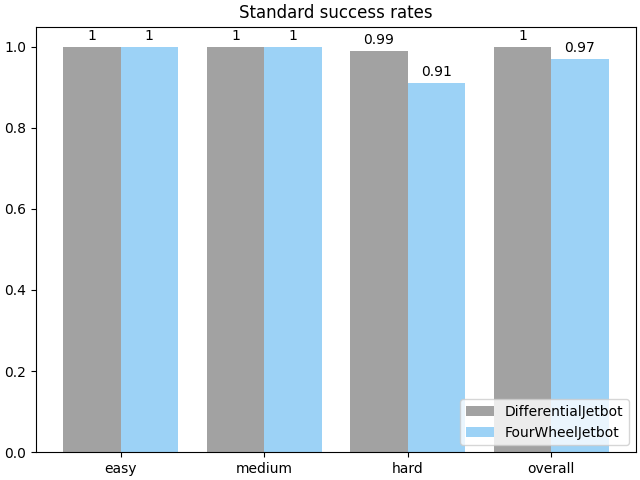
\includegraphics[width=0.45\textwidth]{Bilder/notebook_images/hardDistanceMixedLight_eval_jetbot_generalization_success_rates_barplot.png}
    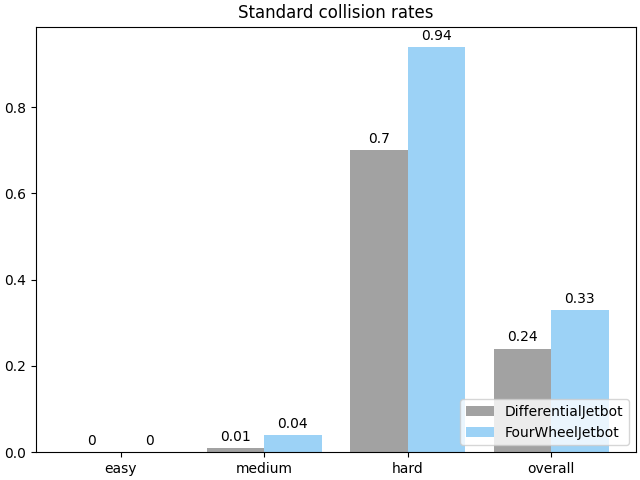
\includegraphics[width=0.45\textwidth]{Bilder/notebook_images/hardDistanceMixedLight_eval_jetbot_generalization_collision_rates_barplot.png}
    \caption{Evaluation of the DifferentialJetBot policy with both jetbot versions}
    \label{fig:result_jetbot_generalization}
\end{figure} % a chart showing the replay outputs

The policy evaluation achieves very high success rates for the FourWheelJetBot with 100\%, 100\% and 91\% for the easy, medium and hard tracks \ref{fig:result_jetbot_generalization}. The collision rates increase for higher difficulties with 0\%, 4\% and 94\%. 
The success and collision rates are slightly worse than on the DifferentialJetBot. The overall success rate of the FourWheelJetBot is 97\% compared to 100\% for the DifferentialJetBot. 

The overall collision rate is 33\% compared to 24\% for the DifferentialJetBot. Especially for the hard tracks the collision rate is much higher for the FourWheelJetBot with 94\% compared to 70\% for the DifferentialJetBot.
The collisions of the DifferentialJetBot were previously described as mainly being minor collisions where the agent scrapes the goal posts with its side. Analysis of the recorded videos shows that the collisions of the FourWheelJetBot are similar. However the agent scrapes the goals on its side for longer durations \ref{sec:fourwheel_collisions}.

% strong collisions here: hard_standard_FourWheelJetBot_env_0_video_2_topview

\paragraph{Discussion}

The policy that was trained on the DifferentialJetBot can be transfered to the FourWheelJetBot with only a slight decrease in performance.
The policy does not have to be retrained in this case. 

